\documentclass[11pt,a4paper]{article}
\usepackage[T1]{fontenc}
\usepackage{graphicx}
\usepackage{hyperref}
\hypersetup{
	colorlinks=true,
	linkcolor=blue,
	filecolor=magenta,      
	urlcolor=blue,
}

\title{Paris Olympics 2024, 100m dash}
\usepackage[legalpaper,  margin=0.5 in]{geometry}

\author{A R Bathri Narayanan, P0211501}
\begin{document}
	\maketitle
	\par\noindent\rule{\textwidth}{0.4pt}
	
	We had seen the Paris Olympics. But one thing that amazed almost everyone was the result of the 100 metre dash. Noah Lyles won the gold medal by five one thousandths of a second. That's the exact time it takes for a bee to flap it's wings!!  How do they measure the timings this accurately? I tried to explore that.
	First let us see how do they measure it usually, with the help of a picture from the internet.\\
	\begin{center}
		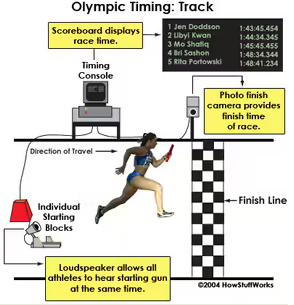
\includegraphics[width=10 cm]{100m1.png}\\
		Olympic conventional clock. Courtesy: HowStuffWorks
	\end{center}
	
	The  first part of the race, is the "gun" to start. This gun is electronic, and is connected to the loudspeaker (So that all racers can hear it almost simultaneously) and to the timing system, to start the timer.\\
	
	The second part, the finish, is done by the camera. The best improvement in modern day Olympics, which saved the day, is the Scan-O-Vision camera or the line scan camera. They have an accuracy of 40000 frames per second. These use digital recording technology. When the leading torso of the runner crosses the line, they record the time and send it to the recording machine. This image is sent to a computer as well, which synchronises the time, and analyses the images sent by it, side by side. Then, it draws a line at each runner's torso at the time the finish line was crossed. This can be obtained within 15 seconds after the race is over.\\

	The image of the actual photo finish is in the next page.
	
	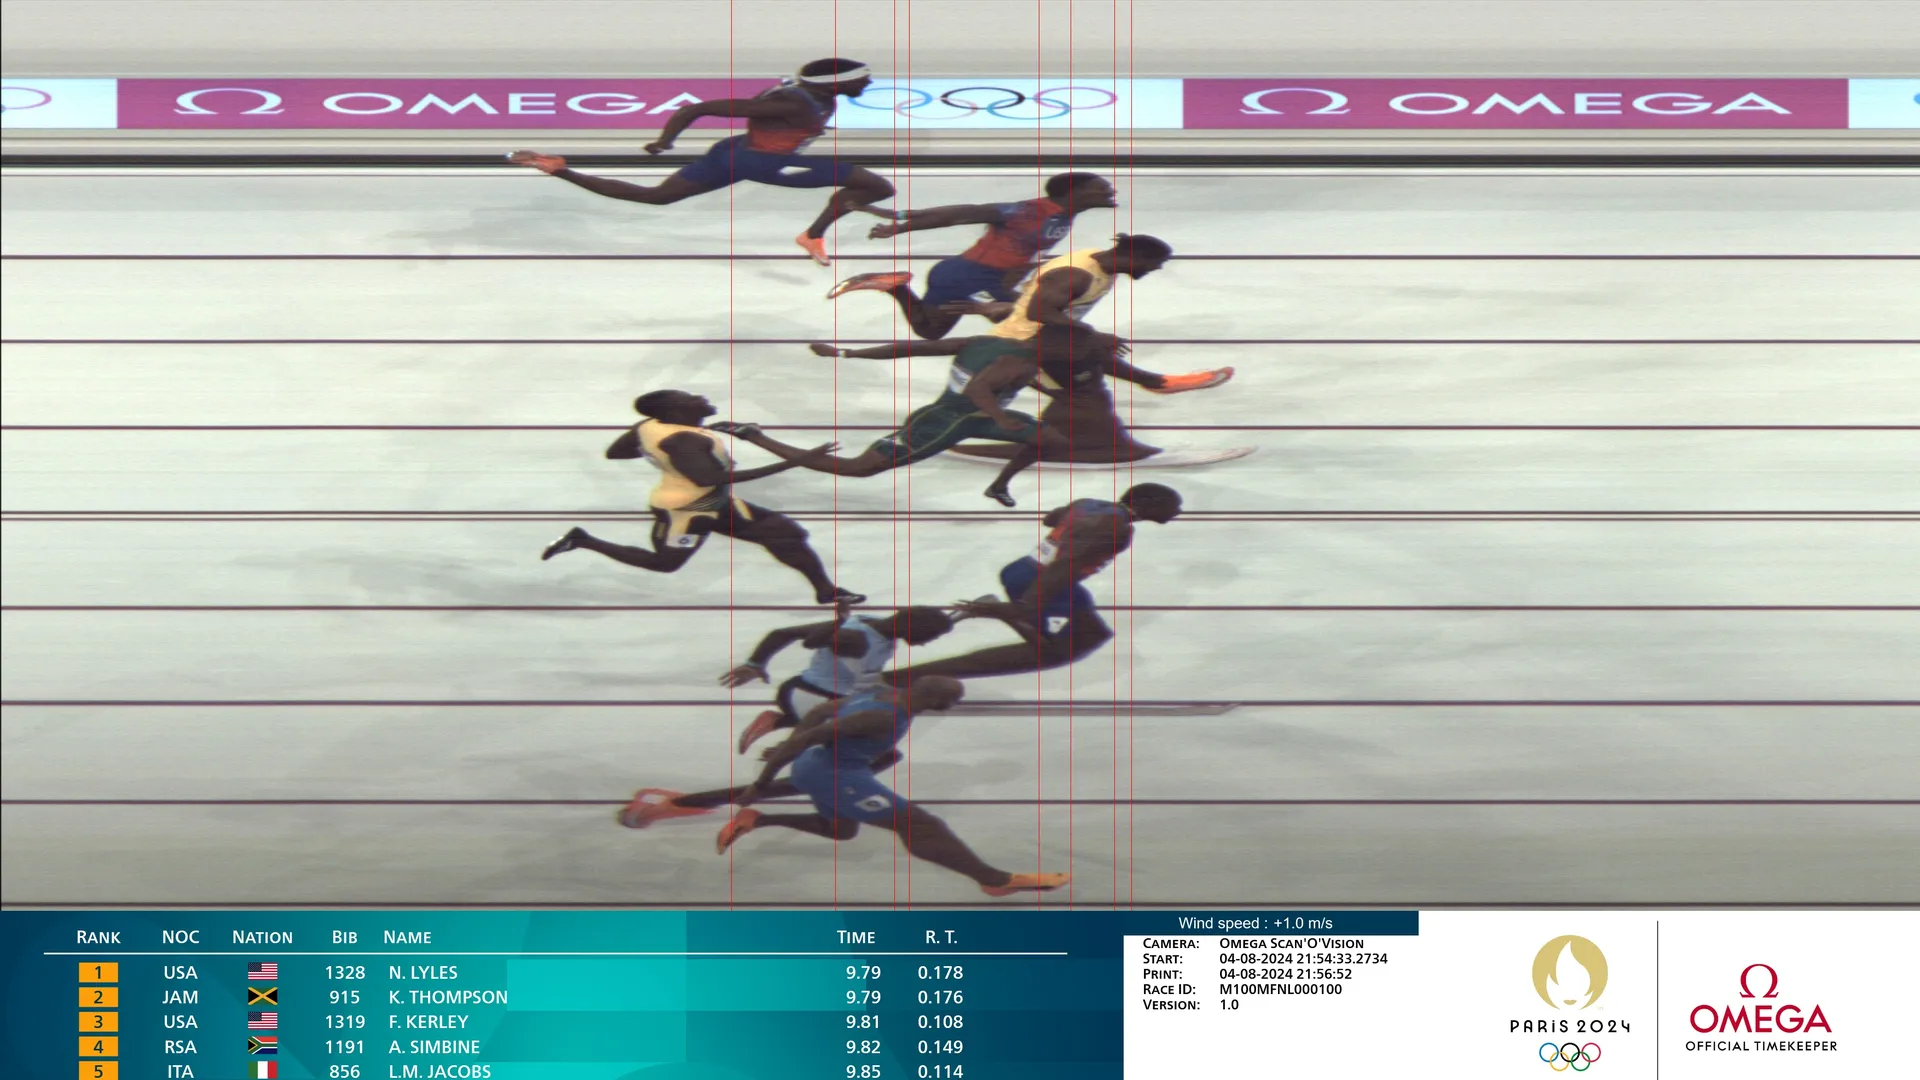
\includegraphics[width=18 cm]{100m2.png}
	\begin{center}
		Photo taken from NBC New York. Credits to Omega, the official timekeeper in Olympics
	\end{center}
	
	We can try to actually calculate the time difference between first and second runner, Kishane Thompson. As you can see, the distance between Lyle's torso and Thompson's torso is about the size of half of Thompson's neck. The average size of human neck is 13 cms. And average speed of Thompson is around 10.13 m/s (100 m in 9.87 seconds). So the math comes out to be
	\[\Delta t = \frac{Distance}{Speed}\approx\frac{0.13 \times 0.5}{10.13}=0.006s\]
	Which is slightly off from the measured 0.005 seconds, but we missed a lot of factors, like the actual height of Thompson's neck, the instantaneous speed of Thompson when he was about to finish (Most athletes decelerate near the finish line) etc. \\
So yes, this result can be believed, thanks to advanced camera techniques.

Now we look at the errors of these measurement devises. The Scan-O-Vision camera has a least count of 1/40000 seconds, which is impressive. 
The possible errors the computer can make are the following.
\begin{itemize}
	\item  Error calculating the distance
	\item Error in identifying the torsos, this can go wrong when they are really close.
	\item Finish line calibration, which won't be a problem with the race, but will be a problem for records like personal best, season best etc.
\end{itemize}
I had also analysed the previous Olympic 100 metre dashes (From 1968 as during 1960 Rome Olympics, the same thing happened (between Armin Hary (GER) and Dave Sime (USA)), and winners were chosen at photo finish which can be sometimes inaccurate) and they come out like this. Note that the time of both of them steadily reduces as years pass due to equipment, new methods of training etc.
\begin{center}
	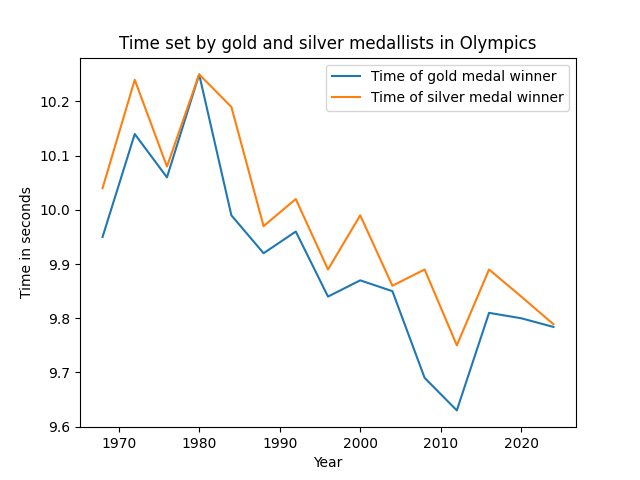
\includegraphics{time.png}
\end{center}

There was one more close finish, at 1980 Moscow Olympics, between Alan Wells (GBR) and Silvio Leonard (CUBA). Again this was sorted by photo finish, but the time was not calculated, both in 1960 and 1978.\\

So compared to both 1960 and 1978, where the photo finish was done based on how much of the body crossed the finish line in the photo, this technique of taking multiple photographs, and getting more accuracy is much more reliable.

\section*{References:} 
\begin{enumerate}
	\item  \href{https://en.wikipedia.org/wiki/Allan_Wells}{Wikipedia page on Alan Wells}
	\item \href{https://www.statista.com/statistics/1090316/olympics-100m-gold-medal-times-since-1896/}{Time points of all gold medal winners, used for verifying the Matplotlib plot}
	\item \href{https://entertainment.howstuffworks.com/olympic-timing.htm}{HowStuffWorks article on timing in Olympics}
	\item \href{https://en.wikipedia.org/wiki/Athletics_at_the_2024_Summer_Olympics_%E2%80%93_Men%27s_100_metres}{Wikipedia page on 2024 100m dash}
	\item \href{https://en.wikipedia.org/wiki/Fully_automatic_time}{Wikipedia article on FAT (Fully Automatic Time)}
\end{enumerate}
	
\end{document}